% ─── Slide: LoRA ablations ────────────────────────────────────────────────────
\begin{frame}[shrink=20]{ADC-LoRA Ablations: Key Findings}
  \begin{columns}[T]
    \begin{column}{0.50\textwidth}
      \textbf{1. CE+KL consistently beats CE}
      \begin{itemize}
        \item \texttt{down+o, r4}: CE $\to$ 15.57; CE+KL $\to$ \better{14.33}
        \item \texttt{all 7, r4}: CE $\to$ 16.68; CE+KL $\to$ \better{14.03}
        \item FP teacher provides signal CE alone cannot
      \end{itemize}
      \vspace{0.2em}
      \textbf{2. Early layers carry more ADC error}
      \begin{itemize}
        \item \texttt{first8}: 16.64 \quad \texttt{last8}: 20.08
        \item Early layers accumulate and \emph{propagate} errors downstream
        \item All 16 layers (r=4, CE+KL): \best{14.03} — best result
      \end{itemize}
      \vspace{0.2em}
      \textbf{3. Post-ADC is the only stable placement}
      \begin{itemize}
        \item Pre-ADC LoRA: no-ADC=123, ADC=105 — catastrophic failure
        \item Gradients through $\texttt{round\_ste}$ are too noisy from step 0
        \item Post-ADC: stable from epoch 1
      \end{itemize}
    \end{column}
    \begin{column}{0.46\textwidth}
      % 4 mini panels
      \iftrue
        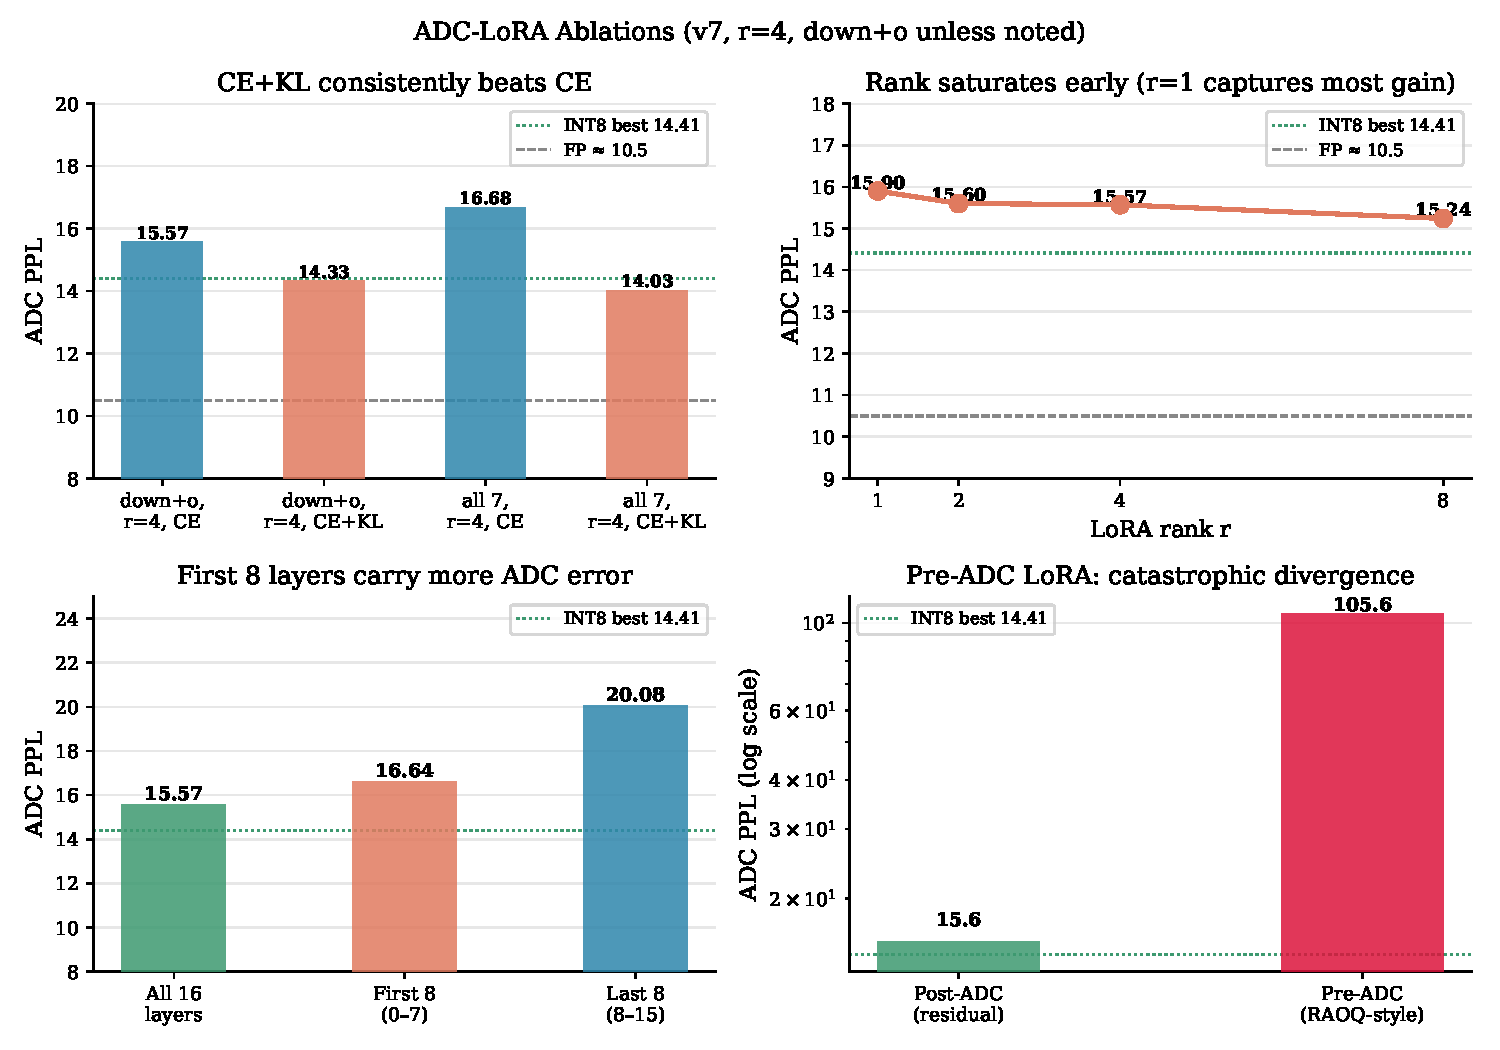
\includegraphics[width=\linewidth]{figs/plot_lora_ablations_grid.pdf}
      \else
        \figplaceholder[0.82\textheight]{2$\times$2 grid of small bar charts.
          Top-left: CE vs CE+KL (down+o and all7).
          Top-right: rank sweep r=1/2/4/8 (down+o, CE+KL).
          Bottom-left: first8 vs last8 vs all16 (ADC PPL).
          Bottom-right: post-ADC vs pre-ADC LoRA — show catastrophic pre-ADC result.}
      \fi
    \end{column}
  \end{columns}
\end{frame}
